\documentclass[1p]{elsarticle_modified}
%\bibliographystyle{elsarticle-num}

%\usepackage[colorlinks]{hyperref}
%\usepackage{abbrmath_seonhwa} %\Abb, \Ascr, \Acal ,\Abf, \Afrak
\usepackage{amsfonts}
\usepackage{amssymb}
\usepackage{amsmath}
\usepackage{amsthm}
\usepackage{scalefnt}
\usepackage{amsbsy}
\usepackage{kotex}
\usepackage{caption}
\usepackage{subfig}
\usepackage{color}
\usepackage{graphicx}
\usepackage{xcolor} %% white, black, red, green, blue, cyan, magenta, yellow
\usepackage{float}
\usepackage{setspace}
\usepackage{hyperref}

\usepackage{tikz}
\usetikzlibrary{arrows}

\usepackage{multirow}
\usepackage{array} % fixed length table
\usepackage{hhline}

%%%%%%%%%%%%%%%%%%%%%
\makeatletter
\renewcommand*\env@matrix[1][\arraystretch]{%
	\edef\arraystretch{#1}%
	\hskip -\arraycolsep
	\let\@ifnextchar\new@ifnextchar
	\array{*\c@MaxMatrixCols c}}
\makeatother %https://tex.stackexchange.com/questions/14071/how-can-i-increase-the-line-spacing-in-a-matrix
%%%%%%%%%%%%%%%

\usepackage[normalem]{ulem}

\newcommand{\msout}[1]{\ifmmode\text{\sout{\ensuremath{#1}}}\else\sout{#1}\fi}
%SOURCE: \msout is \stkout macro in https://tex.stackexchange.com/questions/20609/strikeout-in-math-mode

\newcommand{\cancel}[1]{
	\ifmmode
	{\color{red}\msout{#1}}
	\else
	{\color{red}\sout{#1}}
	\fi
}

\newcommand{\add}[1]{
	{\color{blue}\uwave{#1}}
}

\newcommand{\replace}[2]{
	\ifmmode
	{\color{red}\msout{#1}}{\color{blue}\uwave{#2}}
	\else
	{\color{red}\sout{#1}}{\color{blue}\uwave{#2}}
	\fi
}

\newcommand{\Sol}{\mathcal{S}} %segment
\newcommand{\D}{D} %diagram
\newcommand{\A}{\mathcal{A}} %arc


%%%%%%%%%%%%%%%%%%%%%%%%%%%%%5 test

\def\sl{\operatorname{\textup{SL}}(2,\Cbb)}
\def\psl{\operatorname{\textup{PSL}}(2,\Cbb)}
\def\quan{\mkern 1mu \triangleright \mkern 1mu}

\theoremstyle{definition}
\newtheorem{thm}{Theorem}[section]
\newtheorem{prop}[thm]{Proposition}
\newtheorem{lem}[thm]{Lemma}
\newtheorem{ques}[thm]{Question}
\newtheorem{cor}[thm]{Corollary}
\newtheorem{defn}[thm]{Definition}
\newtheorem{exam}[thm]{Example}
\newtheorem{rmk}[thm]{Remark}
\newtheorem{alg}[thm]{Algorithm}

\newcommand{\I}{\sqrt{-1}}
\begin{document}

%\begin{frontmatter}
%
%\title{Boundary parabolic representations of knots up to 8 crossings}
%
%%% Group authors per affiliation:
%\author{Yunhi Cho} 
%\address{Department of Mathematics, University of Seoul, Seoul, Korea}
%\ead{yhcho@uos.ac.kr}
%
%
%\author{Seonhwa Kim} %\fnref{s_kim}}
%\address{Center for Geometry and Physics, Institute for Basic Science, Pohang, 37673, Korea}
%\ead{ryeona17@ibs.re.kr}
%
%\author{Hyuk Kim}
%\address{Department of Mathematical Sciences, Seoul National University, Seoul 08826, Korea}
%\ead{hyukkim@snu.ac.kr}
%
%\author{Seokbeom Yoon}
%\address{Department of Mathematical Sciences, Seoul National University, Seoul, 08826,  Korea}
%\ead{sbyoon15@snu.ac.kr}
%
%\begin{abstract}
%We find all boundary parabolic representation of knots up to 8 crossings.
%
%\end{abstract}
%\begin{keyword}
%    \MSC[2010] 57M25 
%\end{keyword}
%
%\end{frontmatter}

%\linenumbers
%\tableofcontents
%
\newcommand\colored[1]{\textcolor{white}{\rule[-0.35ex]{0.8em}{1.4ex}}\kern-0.8em\color{red} #1}%
%\newcommand\colored[1]{\textcolor{white}{ #1}\kern-2.17ex	\textcolor{white}{ #1}\kern-1.81ex	\textcolor{white}{ #1}\kern-2.15ex\color{red}#1	}

{\Large $\underline{12a_{0026}~(K12a_{0026})}$}

\setlength{\tabcolsep}{10pt}
\renewcommand{\arraystretch}{1.6}
\vspace{1cm}\begin{tabular}{m{100pt}>{\centering\arraybackslash}m{274pt}}
\multirow{5}{120pt}{
	\centering
	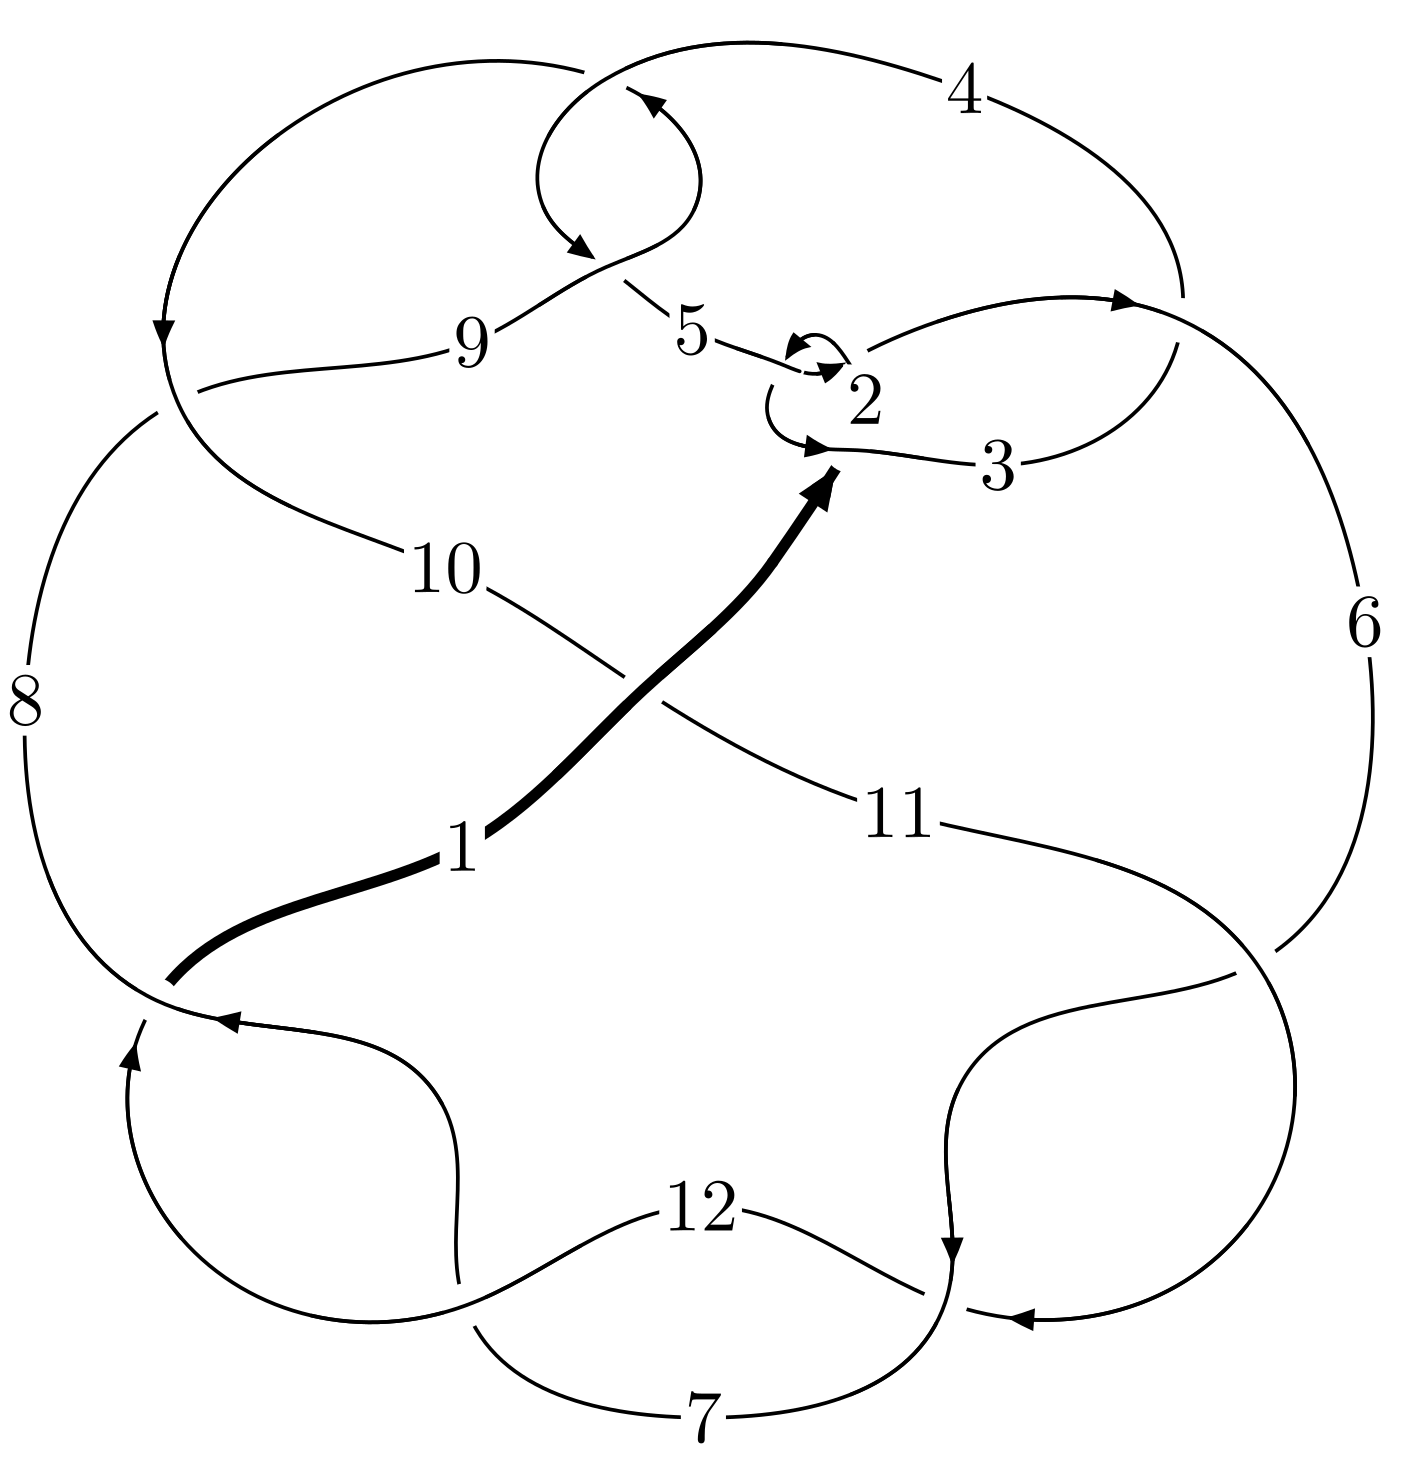
\includegraphics[width=112pt]{../../../GIT/diagram.site/Diagrams/png/827_12a_0026.png}\\
\ \ \ A knot diagram\footnotemark}&
\allowdisplaybreaks
\textbf{Linearized knot diagam} \\
\cline{2-2}
 &
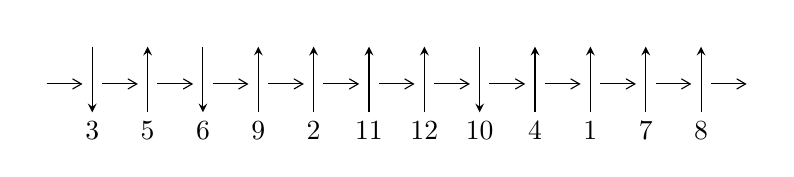
\begin{tikzpicture}[x=20pt, y=17pt]
	% nodes
	\node (C0) at (0, 0) {};
	\node (C1) at (1, 0) {};
	\node (C1U) at (1, +1) {};
	\node (C1D) at (1, -1) {3};

	\node (C2) at (2, 0) {};
	\node (C2U) at (2, +1) {};
	\node (C2D) at (2, -1) {5};

	\node (C3) at (3, 0) {};
	\node (C3U) at (3, +1) {};
	\node (C3D) at (3, -1) {6};

	\node (C4) at (4, 0) {};
	\node (C4U) at (4, +1) {};
	\node (C4D) at (4, -1) {9};

	\node (C5) at (5, 0) {};
	\node (C5U) at (5, +1) {};
	\node (C5D) at (5, -1) {2};

	\node (C6) at (6, 0) {};
	\node (C6U) at (6, +1) {};
	\node (C6D) at (6, -1) {11};

	\node (C7) at (7, 0) {};
	\node (C7U) at (7, +1) {};
	\node (C7D) at (7, -1) {12};

	\node (C8) at (8, 0) {};
	\node (C8U) at (8, +1) {};
	\node (C8D) at (8, -1) {10};

	\node (C9) at (9, 0) {};
	\node (C9U) at (9, +1) {};
	\node (C9D) at (9, -1) {4};

	\node (C10) at (10, 0) {};
	\node (C10U) at (10, +1) {};
	\node (C10D) at (10, -1) {1};

	\node (C11) at (11, 0) {};
	\node (C11U) at (11, +1) {};
	\node (C11D) at (11, -1) {7};

	\node (C12) at (12, 0) {};
	\node (C12U) at (12, +1) {};
	\node (C12D) at (12, -1) {8};
	\node (C13) at (13, 0) {};

	% arrows
	\draw[->,>={angle 60}]
	(C0) edge (C1) (C1) edge (C2) (C2) edge (C3) (C3) edge (C4) (C4) edge (C5) (C5) edge (C6) (C6) edge (C7) (C7) edge (C8) (C8) edge (C9) (C9) edge (C10) (C10) edge (C11) (C11) edge (C12) (C12) edge (C13) ;	\draw[->,>=stealth]
	(C1U) edge (C1D) (C2D) edge (C2U) (C3U) edge (C3D) (C4D) edge (C4U) (C5D) edge (C5U) (C6D) edge (C6U) (C7D) edge (C7U) (C8U) edge (C8D) (C9D) edge (C9U) (C10D) edge (C10U) (C11D) edge (C11U) (C12D) edge (C12U) ;
	\end{tikzpicture} \\
\hhline{~~} \\& 
\textbf{Solving Sequence} \\ \cline{2-2} 
 &
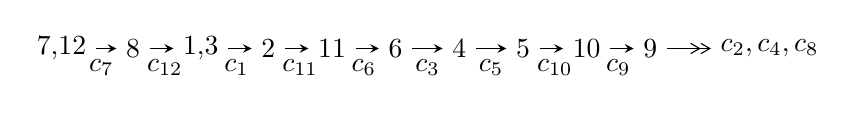
\begin{tikzpicture}[x=23pt, y=7pt]
	% node
	\node (A0) at (-1/8, 0) {7,12};
	\node (A1) at (1, 0) {8};
	\node (A2) at (33/16, 0) {1,3};
	\node (A3) at (25/8, 0) {2};
	\node (A4) at (33/8, 0) {11};
	\node (A5) at (41/8, 0) {6};
	\node (A6) at (49/8, 0) {4};
	\node (A7) at (57/8, 0) {5};
	\node (A8) at (65/8, 0) {10};
	\node (A9) at (73/8, 0) {9};
	\node (C1) at (1/2, -1) {$c_{7}$};
	\node (C2) at (3/2, -1) {$c_{12}$};
	\node (C3) at (21/8, -1) {$c_{1}$};
	\node (C4) at (29/8, -1) {$c_{11}$};
	\node (C5) at (37/8, -1) {$c_{6}$};
	\node (C6) at (45/8, -1) {$c_{3}$};
	\node (C7) at (53/8, -1) {$c_{5}$};
	\node (C8) at (61/8, -1) {$c_{10}$};
	\node (C9) at (69/8, -1) {$c_{9}$};
	\node (A10) at (11, 0) {$c_{2},c_{4},c_{8}$};

	% edge
	\draw[->,>=stealth]	
	(A0) edge (A1) (A1) edge (A2) (A2) edge (A3) (A3) edge (A4) (A4) edge (A5) (A5) edge (A6) (A6) edge (A7) (A7) edge (A8) (A8) edge (A9) ;
	\draw[->>,>={angle 60}]	
	(A9) edge (A10);
\end{tikzpicture} \\ 

\end{tabular} \\

\footnotetext{
The image of knot diagram is generated by the software ``\textbf{Draw programme}" developed by Andrew Bartholomew(\url{http://www.layer8.co.uk/maths/draw/index.htm\#Running-draw}), where we modified some parts for our purpose(\url{https://github.com/CATsTAILs/LinksPainter}).
}\phantom \\ \newline 
\centering \textbf{Ideals for irreducible components\footnotemark of $X_{\text{par}}$} 
 
\begin{align*}
I^u_{1}&=\langle 
15 u^{75}+20 u^{74}+\cdots+2 b-12,\;-3 u^{75}+135 u^{73}+\cdots+2 a+8,\;u^{76}+3 u^{75}+\cdots+2 u-1\rangle \\
I^u_{2}&=\langle 
b+a,\;a^2- a+1,\;u^2- u-1\rangle \\
\\
\end{align*}
\raggedright * 2 irreducible components of $\dim_{\mathbb{C}}=0$, with total 80 representations.\\
\footnotetext{All coefficients of polynomials are rational numbers. But the coefficients are sometimes approximated in decimal forms when there is not enough margin.}
\newpage
\renewcommand{\arraystretch}{1}
\centering \section*{I. $I^u_{1}= \langle 15 u^{75}+20 u^{74}+\cdots+2 b-12,\;-3 u^{75}+135 u^{73}+\cdots+2 a+8,\;u^{76}+3 u^{75}+\cdots+2 u-1 \rangle$}
\flushleft \textbf{(i) Arc colorings}\\
\begin{tabular}{m{7pt} m{180pt} m{7pt} m{180pt} }
\flushright $a_{7}=$&$\begin{pmatrix}1\\0\end{pmatrix}$ \\
\flushright $a_{12}=$&$\begin{pmatrix}0\\u\end{pmatrix}$ \\
\flushright $a_{8}=$&$\begin{pmatrix}1\\- u^2\end{pmatrix}$ \\
\flushright $a_{1}=$&$\begin{pmatrix}u\\- u^3+u\end{pmatrix}$ \\
\flushright $a_{3}=$&$\begin{pmatrix}\frac{3}{2} u^{75}-\frac{135}{2} u^{73}+\cdots+\frac{11}{2} u-4\\-\frac{15}{2} u^{75}-10 u^{74}+\cdots-\frac{25}{2} u+6\end{pmatrix}$ \\
\flushright $a_{2}=$&$\begin{pmatrix}-\frac{1}{2} u^{75}- u^{74}+\cdots+\frac{3}{2} u+1\\\frac{1}{2} u^{75}+u^{74}+\cdots-\frac{3}{2} u^2+\frac{1}{2} u\end{pmatrix}$ \\
\flushright $a_{11}=$&$\begin{pmatrix}- u\\u\end{pmatrix}$ \\
\flushright $a_{6}=$&$\begin{pmatrix}- u^2+1\\u^2\end{pmatrix}$ \\
\flushright $a_{4}=$&$\begin{pmatrix}8 u^{75}+\frac{17}{2} u^{74}+\cdots+\frac{33}{2} u-\frac{19}{2}\\-\frac{39}{2} u^{75}-\frac{55}{2} u^{74}+\cdots-33 u+\frac{27}{2}\end{pmatrix}$ \\
\flushright $a_{5}=$&$\begin{pmatrix}6 u^{75}+\frac{21}{2} u^{74}+\cdots+\frac{17}{2} u-\frac{1}{2}\\-\frac{9}{2} u^{75}-\frac{15}{2} u^{74}+\cdots-7 u+\frac{3}{2}\end{pmatrix}$ \\
\flushright $a_{10}=$&$\begin{pmatrix}u^5-2 u^3- u\\- u^7+3 u^5-2 u^3+u\end{pmatrix}$ \\
\flushright $a_{9}=$&$\begin{pmatrix}u^{10}-5 u^8+6 u^6+u^4- u^2+1\\- u^{12}+6 u^{10}-12 u^8+10 u^6-5 u^4\end{pmatrix}$\\&\end{tabular}
\flushleft \textbf{(ii) Obstruction class $= -1$}\\~\\
\flushleft \textbf{(iii) Cusp Shapes $= \frac{29}{2} u^{75}+24 u^{74}+\cdots+\frac{13}{2} u+1$}\\~\\
\newpage\renewcommand{\arraystretch}{1}
\flushleft \textbf{(iv) u-Polynomials at the component}\newline \\
\begin{tabular}{m{50pt}|m{274pt}}
Crossings & \hspace{64pt}u-Polynomials at each crossing \\
\hline $$\begin{aligned}c_{1}\end{aligned}$$&$\begin{aligned}
&u^{76}+35 u^{75}+\cdots-34 u+1
\end{aligned}$\\
\hline $$\begin{aligned}c_{2},c_{5}\end{aligned}$$&$\begin{aligned}
&u^{76}+3 u^{75}+\cdots-2 u+1
\end{aligned}$\\
\hline $$\begin{aligned}c_{3}\end{aligned}$$&$\begin{aligned}
&u^{76}-3 u^{75}+\cdots-458 u+41
\end{aligned}$\\
\hline $$\begin{aligned}c_{4},c_{9}\end{aligned}$$&$\begin{aligned}
&u^{76}+u^{75}+\cdots-124 u^2-16
\end{aligned}$\\
\hline $$\begin{aligned}c_{6},c_{7},c_{11}\\c_{12}\end{aligned}$$&$\begin{aligned}
&u^{76}-3 u^{75}+\cdots-2 u-1
\end{aligned}$\\
\hline $$\begin{aligned}c_{8}\end{aligned}$$&$\begin{aligned}
&u^{76}+25 u^{75}+\cdots+3968 u+256
\end{aligned}$\\
\hline $$\begin{aligned}c_{10}\end{aligned}$$&$\begin{aligned}
&u^{76}+23 u^{75}+\cdots-53922 u-8023
\end{aligned}$\\
\hline
\end{tabular}\\~\\
\newpage\renewcommand{\arraystretch}{1}
\flushleft \textbf{(v) Riley Polynomials at the component}\newline \\
\begin{tabular}{m{50pt}|m{274pt}}
Crossings & \hspace{64pt}Riley Polynomials at each crossing \\
\hline $$\begin{aligned}c_{1}\end{aligned}$$&$\begin{aligned}
&y^{76}+15 y^{75}+\cdots-1370 y+1
\end{aligned}$\\
\hline $$\begin{aligned}c_{2},c_{5}\end{aligned}$$&$\begin{aligned}
&y^{76}+35 y^{75}+\cdots-34 y+1
\end{aligned}$\\
\hline $$\begin{aligned}c_{3}\end{aligned}$$&$\begin{aligned}
&y^{76}-5 y^{75}+\cdots-135554 y+1681
\end{aligned}$\\
\hline $$\begin{aligned}c_{4},c_{9}\end{aligned}$$&$\begin{aligned}
&y^{76}+25 y^{75}+\cdots+3968 y+256
\end{aligned}$\\
\hline $$\begin{aligned}c_{6},c_{7},c_{11}\\c_{12}\end{aligned}$$&$\begin{aligned}
&y^{76}-89 y^{75}+\cdots-14 y+1
\end{aligned}$\\
\hline $$\begin{aligned}c_{8}\end{aligned}$$&$\begin{aligned}
&y^{76}+45 y^{75}+\cdots-4202496 y+65536
\end{aligned}$\\
\hline $$\begin{aligned}c_{10}\end{aligned}$$&$\begin{aligned}
&y^{76}-29 y^{75}+\cdots-1605176402 y+64368529
\end{aligned}$\\
\hline
\end{tabular}\\~\\
\newpage\flushleft \textbf{(vi) Complex Volumes and Cusp Shapes}
$$\begin{array}{c|c|c}  
\text{Solutions to }I^u_{1}& \I (\text{vol} + \sqrt{-1}CS) & \text{Cusp shape}\\
 \hline 
\begin{aligned}
u &= -0.885990 + 0.333160 I \\
a &= \phantom{-}0.872634 - 0.542118 I \\
b &= -0.67077 + 1.24857 I\end{aligned}
 & \phantom{-}1.97205 + 5.49296 I & \phantom{-0.000000 } 0 \\ \hline\begin{aligned}
u &= -0.885990 - 0.333160 I \\
a &= \phantom{-}0.872634 + 0.542118 I \\
b &= -0.67077 - 1.24857 I\end{aligned}
 & \phantom{-}1.97205 - 5.49296 I & \phantom{-0.000000 } 0 \\ \hline\begin{aligned}
u &= \phantom{-}0.751786 + 0.507447 I \\
a &= -1.107940 - 0.282272 I \\
b &= -0.99521 - 1.10936 I\end{aligned}
 & \phantom{-}0.67458 + 12.58000 I & \phantom{-0.000000 } 0 \\ \hline\begin{aligned}
u &= \phantom{-}0.751786 - 0.507447 I \\
a &= -1.107940 + 0.282272 I \\
b &= -0.99521 + 1.10936 I\end{aligned}
 & \phantom{-}0.67458 - 12.58000 I & \phantom{-0.000000 } 0 \\ \hline\begin{aligned}
u &= -0.836373 + 0.339607 I \\
a &= -0.755203 + 0.432767 I \\
b &= -0.004969 - 0.761767 I\end{aligned}
 & \phantom{-}3.83321 + 0.59439 I & \phantom{-0.000000 } 0 \\ \hline\begin{aligned}
u &= -0.836373 - 0.339607 I \\
a &= -0.755203 - 0.432767 I \\
b &= -0.004969 + 0.761767 I\end{aligned}
 & \phantom{-}3.83321 - 0.59439 I & \phantom{-0.000000 } 0 \\ \hline\begin{aligned}
u &= \phantom{-}0.747341 + 0.484979 I \\
a &= \phantom{-}0.910922 + 0.390103 I \\
b &= \phantom{-}0.844895 + 0.477346 I\end{aligned}
 & \phantom{-}2.79991 + 7.37350 I & \phantom{-0.000000 } 0 \\ \hline\begin{aligned}
u &= \phantom{-}0.747341 - 0.484979 I \\
a &= \phantom{-}0.910922 - 0.390103 I \\
b &= \phantom{-}0.844895 - 0.477346 I\end{aligned}
 & \phantom{-}2.79991 - 7.37350 I & \phantom{-0.000000 } 0 \\ \hline\begin{aligned}
u &= -0.867041 + 0.154083 I \\
a &= \phantom{-}0.590113 + 0.095531 I \\
b &= -0.737271 - 0.597559 I\end{aligned}
 & -0.213421 - 1.034600 I & \phantom{-0.000000 } 0 \\ \hline\begin{aligned}
u &= -0.867041 - 0.154083 I \\
a &= \phantom{-}0.590113 - 0.095531 I \\
b &= -0.737271 + 0.597559 I\end{aligned}
 & -0.213421 + 1.034600 I & \phantom{-0.000000 } 0\\
 \hline 
 \end{array}$$\newpage$$\begin{array}{c|c|c}  
\text{Solutions to }I^u_{1}& \I (\text{vol} + \sqrt{-1}CS) & \text{Cusp shape}\\
 \hline 
\begin{aligned}
u &= \phantom{-}0.694227 + 0.488418 I \\
a &= -0.862705 - 0.739564 I \\
b &= \phantom{-}0.268689 - 0.485835 I\end{aligned}
 & -2.20786 + 5.00695 I & \phantom{-0.000000 } 0 \\ \hline\begin{aligned}
u &= \phantom{-}0.694227 - 0.488418 I \\
a &= -0.862705 + 0.739564 I \\
b &= \phantom{-}0.268689 + 0.485835 I\end{aligned}
 & -2.20786 - 5.00695 I & \phantom{-0.000000 } 0 \\ \hline\begin{aligned}
u &= \phantom{-}0.740484 + 0.411101 I \\
a &= \phantom{-}0.765867 + 0.569492 I \\
b &= \phantom{-}0.136180 - 0.867389 I\end{aligned}
 & \phantom{-}3.76796 + 4.58951 I & \phantom{-0.000000 } 0 \\ \hline\begin{aligned}
u &= \phantom{-}0.740484 - 0.411101 I \\
a &= \phantom{-}0.765867 - 0.569492 I \\
b &= \phantom{-}0.136180 + 0.867389 I\end{aligned}
 & \phantom{-}3.76796 - 4.58951 I & \phantom{-0.000000 } 0 \\ \hline\begin{aligned}
u &= -0.745942 + 0.396837 I \\
a &= -1.022130 + 0.377114 I \\
b &= -0.892114 + 0.438279 I\end{aligned}
 & \phantom{-}3.86486 - 1.58644 I & \phantom{-0.000000 } 0 \\ \hline\begin{aligned}
u &= -0.745942 - 0.396837 I \\
a &= -1.022130 - 0.377114 I \\
b &= -0.892114 - 0.438279 I\end{aligned}
 & \phantom{-}3.86486 + 1.58644 I & \phantom{-0.000000 } 0 \\ \hline\begin{aligned}
u &= -0.719638 + 0.432491 I \\
a &= \phantom{-}1.39607 - 0.37314 I \\
b &= \phantom{-}1.09423 - 1.13795 I\end{aligned}
 & \phantom{-}2.04591 - 6.50107 I & \phantom{-0.000000 } 0 \\ \hline\begin{aligned}
u &= -0.719638 - 0.432491 I \\
a &= \phantom{-}1.39607 + 0.37314 I \\
b &= \phantom{-}1.09423 + 1.13795 I\end{aligned}
 & \phantom{-}2.04591 + 6.50107 I & \phantom{-0.000000 } 0 \\ \hline\begin{aligned}
u &= \phantom{-}0.731033 + 0.364174 I \\
a &= -0.925187 - 0.555287 I \\
b &= \phantom{-}0.510713 + 1.186120 I\end{aligned}
 & \phantom{-}2.50490 - 0.55456 I & \phantom{-}9.61533 - 2.91728 I \\ \hline\begin{aligned}
u &= \phantom{-}0.731033 - 0.364174 I \\
a &= -0.925187 + 0.555287 I \\
b &= \phantom{-}0.510713 - 1.186120 I\end{aligned}
 & \phantom{-}2.50490 + 0.55456 I & \phantom{-}9.61533 + 2.91728 I\\
 \hline 
 \end{array}$$\newpage$$\begin{array}{c|c|c}  
\text{Solutions to }I^u_{1}& \I (\text{vol} + \sqrt{-1}CS) & \text{Cusp shape}\\
 \hline 
\begin{aligned}
u &= \phantom{-}0.505111 + 0.534579 I \\
a &= -1.202510 + 0.531702 I \\
b &= -0.942344 - 0.780413 I\end{aligned}
 & -5.36892 + 5.69274 I & \phantom{-}0.38490 - 7.89158 I \\ \hline\begin{aligned}
u &= \phantom{-}0.505111 - 0.534579 I \\
a &= -1.202510 - 0.531702 I \\
b &= -0.942344 + 0.780413 I\end{aligned}
 & -5.36892 - 5.69274 I & \phantom{-}0.38490 + 7.89158 I \\ \hline\begin{aligned}
u &= -0.596247 + 0.341693 I \\
a &= \phantom{-}0.55214 - 1.30810 I \\
b &= -0.441166 - 0.807337 I\end{aligned}
 & -0.315070 - 0.076640 I & \phantom{-}5.64186 + 2.36469 I \\ \hline\begin{aligned}
u &= -0.596247 - 0.341693 I \\
a &= \phantom{-}0.55214 + 1.30810 I \\
b &= -0.441166 + 0.807337 I\end{aligned}
 & -0.315070 + 0.076640 I & \phantom{-}5.64186 - 2.36469 I \\ \hline\begin{aligned}
u &= \phantom{-}0.404061 + 0.546779 I \\
a &= -1.53472 - 0.82950 I \\
b &= -0.103415 - 0.768073 I\end{aligned}
 & -5.65998 - 1.97285 I & -0.963134 + 0.338595 I \\ \hline\begin{aligned}
u &= \phantom{-}0.404061 - 0.546779 I \\
a &= -1.53472 + 0.82950 I \\
b &= -0.103415 + 0.768073 I\end{aligned}
 & -5.65998 + 1.97285 I & -0.963134 - 0.338595 I \\ \hline\begin{aligned}
u &= \phantom{-}0.456233 + 0.476408 I \\
a &= \phantom{-}0.807953 + 0.259709 I \\
b &= \phantom{-}0.581862 + 0.454575 I\end{aligned}
 & -2.40945 + 1.67574 I & \phantom{-}3.56432 - 4.46273 I \\ \hline\begin{aligned}
u &= \phantom{-}0.456233 - 0.476408 I \\
a &= \phantom{-}0.807953 - 0.259709 I \\
b &= \phantom{-}0.581862 - 0.454575 I\end{aligned}
 & -2.40945 - 1.67574 I & \phantom{-}3.56432 + 4.46273 I \\ \hline\begin{aligned}
u &= \phantom{-}0.121254 + 0.636401 I \\
a &= -1.82213 - 0.10923 I \\
b &= -0.352065 - 0.838752 I\end{aligned}
 & -1.18944 - 8.72098 I & \phantom{-}3.35149 + 6.41865 I \\ \hline\begin{aligned}
u &= \phantom{-}0.121254 - 0.636401 I \\
a &= -1.82213 + 0.10923 I \\
b &= -0.352065 + 0.838752 I\end{aligned}
 & -1.18944 + 8.72098 I & \phantom{-}3.35149 - 6.41865 I\\
 \hline 
 \end{array}$$\newpage$$\begin{array}{c|c|c}  
\text{Solutions to }I^u_{1}& \I (\text{vol} + \sqrt{-1}CS) & \text{Cusp shape}\\
 \hline 
\begin{aligned}
u &= \phantom{-}0.105876 + 0.603977 I \\
a &= \phantom{-}0.938724 + 0.288370 I \\
b &= \phantom{-}0.264725 + 0.759368 I\end{aligned}
 & \phantom{-}0.91644 - 3.68473 I & \phantom{-}6.38251 + 2.47980 I \\ \hline\begin{aligned}
u &= \phantom{-}0.105876 - 0.603977 I \\
a &= \phantom{-}0.938724 - 0.288370 I \\
b &= \phantom{-}0.264725 - 0.759368 I\end{aligned}
 & \phantom{-}0.91644 + 3.68473 I & \phantom{-}6.38251 - 2.47980 I \\ \hline\begin{aligned}
u &= \phantom{-}0.187489 + 0.573478 I \\
a &= -0.431525 + 1.144150 I \\
b &= -0.402625 - 0.455153 I\end{aligned}
 & -3.68972 - 1.37288 I & -0.612694 + 0.508979 I \\ \hline\begin{aligned}
u &= \phantom{-}0.187489 - 0.573478 I \\
a &= -0.431525 - 1.144150 I \\
b &= -0.402625 + 0.455153 I\end{aligned}
 & -3.68972 + 1.37288 I & -0.612694 - 0.508979 I \\ \hline\begin{aligned}
u &= -1.46039 + 0.08103 I \\
a &= \phantom{-}1.46326 - 1.34448 I \\
b &= -2.15619 + 2.33527 I\end{aligned}
 & \phantom{-}0.265608 - 0.146440 I & \phantom{-0.000000 } 0 \\ \hline\begin{aligned}
u &= -1.46039 - 0.08103 I \\
a &= \phantom{-}1.46326 + 1.34448 I \\
b &= -2.15619 - 2.33527 I\end{aligned}
 & \phantom{-}0.265608 + 0.146440 I & \phantom{-0.000000 } 0 \\ \hline\begin{aligned}
u &= \phantom{-}0.013313 + 0.514387 I \\
a &= -1.138510 + 0.344338 I \\
b &= -0.070209 + 0.768340 I\end{aligned}
 & \phantom{-}1.70461 - 1.46252 I & \phantom{-}7.24578 + 3.00546 I \\ \hline\begin{aligned}
u &= \phantom{-}0.013313 - 0.514387 I \\
a &= -1.138510 - 0.344338 I \\
b &= -0.070209 - 0.768340 I\end{aligned}
 & \phantom{-}1.70461 + 1.46252 I & \phantom{-}7.24578 - 3.00546 I \\ \hline\begin{aligned}
u &= -0.082708 + 0.494197 I \\
a &= \phantom{-}2.30376 - 0.01004 I \\
b &= \phantom{-}0.338632 - 0.907658 I\end{aligned}
 & \phantom{-}0.24315 + 3.28654 I & \phantom{-}4.66258 - 2.10063 I \\ \hline\begin{aligned}
u &= -0.082708 - 0.494197 I \\
a &= \phantom{-}2.30376 + 0.01004 I \\
b &= \phantom{-}0.338632 + 0.907658 I\end{aligned}
 & \phantom{-}0.24315 - 3.28654 I & \phantom{-}4.66258 + 2.10063 I\\
 \hline 
 \end{array}$$\newpage$$\begin{array}{c|c|c}  
\text{Solutions to }I^u_{1}& \I (\text{vol} + \sqrt{-1}CS) & \text{Cusp shape}\\
 \hline 
\begin{aligned}
u &= -1.50687 + 0.12545 I \\
a &= \phantom{-}2.62859 - 0.35369 I \\
b &= -3.79993 + 0.65614 I\end{aligned}
 & \phantom{-}1.23477 - 8.00671 I & \phantom{-0.000000 } 0 \\ \hline\begin{aligned}
u &= -1.50687 - 0.12545 I \\
a &= \phantom{-}2.62859 + 0.35369 I \\
b &= -3.79993 - 0.65614 I\end{aligned}
 & \phantom{-}1.23477 + 8.00671 I & \phantom{-0.000000 } 0 \\ \hline\begin{aligned}
u &= -1.50985 + 0.09146 I \\
a &= -1.82204 + 0.35941 I \\
b &= \phantom{-}2.53314 - 0.79410 I\end{aligned}
 & \phantom{-}4.06697 - 3.56308 I & \phantom{-0.000000 } 0 \\ \hline\begin{aligned}
u &= -1.50985 - 0.09146 I \\
a &= -1.82204 - 0.35941 I \\
b &= \phantom{-}2.53314 + 0.79410 I\end{aligned}
 & \phantom{-}4.06697 + 3.56308 I & \phantom{-0.000000 } 0 \\ \hline\begin{aligned}
u &= -0.485277\phantom{ +0.000000I} \\
a &= -0.607470\phantom{ +0.000000I} \\
b &= -0.408478\phantom{ +0.000000I}\end{aligned}
 & \phantom{-}0.739641\phantom{ +0.000000I} & \phantom{-}13.5000\phantom{ +0.000000I} \\ \hline\begin{aligned}
u &= -0.332468 + 0.348514 I \\
a &= \phantom{-}1.46781 + 1.80245 I \\
b &= \phantom{-}1.019820 - 0.128661 I\end{aligned}
 & -1.06070 - 2.50916 I & \phantom{-}3.18547 + 6.68598 I \\ \hline\begin{aligned}
u &= -0.332468 - 0.348514 I \\
a &= \phantom{-}1.46781 - 1.80245 I \\
b &= \phantom{-}1.019820 + 0.128661 I\end{aligned}
 & -1.06070 + 2.50916 I & \phantom{-}3.18547 - 6.68598 I \\ \hline\begin{aligned}
u &= \phantom{-}1.51846 + 0.03177 I \\
a &= -3.24068 + 1.10209 I \\
b &= \phantom{-}4.94954 - 1.73737 I\end{aligned}
 & \phantom{-}5.15855 + 3.46829 I & \phantom{-0.000000 } 0 \\ \hline\begin{aligned}
u &= \phantom{-}1.51846 - 0.03177 I \\
a &= -3.24068 - 1.10209 I \\
b &= \phantom{-}4.94954 + 1.73737 I\end{aligned}
 & \phantom{-}5.15855 - 3.46829 I & \phantom{-0.000000 } 0 \\ \hline\begin{aligned}
u &= -1.54556 + 0.01387 I \\
a &= -0.439333 - 0.753773 I \\
b &= \phantom{-}0.502805 + 0.325969 I\end{aligned}
 & \phantom{-}7.25856 - 2.56091 I & \phantom{-0.000000 } 0\\
 \hline 
 \end{array}$$\newpage$$\begin{array}{c|c|c}  
\text{Solutions to }I^u_{1}& \I (\text{vol} + \sqrt{-1}CS) & \text{Cusp shape}\\
 \hline 
\begin{aligned}
u &= -1.54556 - 0.01387 I \\
a &= -0.439333 + 0.753773 I \\
b &= \phantom{-}0.502805 - 0.325969 I\end{aligned}
 & \phantom{-}7.25856 + 2.56091 I & \phantom{-0.000000 } 0 \\ \hline\begin{aligned}
u &= \phantom{-}1.55696\phantom{ +0.000000I} \\
a &= \phantom{-}2.02517\phantom{ +0.000000I} \\
b &= -3.03221\phantom{ +0.000000I}\end{aligned}
 & \phantom{-}7.77426\phantom{ +0.000000I} & \phantom{-0.000000 } 0 \\ \hline\begin{aligned}
u &= \phantom{-}0.398202 + 0.093446 I \\
a &= -0.14340 + 1.82967 I \\
b &= \phantom{-}0.405564 - 0.876916 I\end{aligned}
 & \phantom{-}0.51331 + 2.24257 I & -1.43172 - 6.93184 I \\ \hline\begin{aligned}
u &= \phantom{-}0.398202 - 0.093446 I \\
a &= -0.14340 - 1.82967 I \\
b &= \phantom{-}0.405564 + 0.876916 I\end{aligned}
 & \phantom{-}0.51331 - 2.24257 I & -1.43172 + 6.93184 I \\ \hline\begin{aligned}
u &= \phantom{-}1.59191 + 0.09160 I \\
a &= -0.24009 - 2.06938 I \\
b &= \phantom{-}0.42940 + 3.38884 I\end{aligned}
 & \phantom{-}7.23380 + 1.61258 I & \phantom{-0.000000 } 0 \\ \hline\begin{aligned}
u &= \phantom{-}1.59191 - 0.09160 I \\
a &= -0.24009 + 2.06938 I \\
b &= \phantom{-}0.42940 - 3.38884 I\end{aligned}
 & \phantom{-}7.23380 - 1.61258 I & \phantom{-0.000000 } 0 \\ \hline\begin{aligned}
u &= -1.60359 + 0.14007 I \\
a &= \phantom{-}0.34694 - 1.56141 I \\
b &= -0.66188 + 2.68266 I\end{aligned}
 & \phantom{-}5.58997 - 7.33867 I & \phantom{-0.000000 } 0 \\ \hline\begin{aligned}
u &= -1.60359 - 0.14007 I \\
a &= \phantom{-}0.34694 + 1.56141 I \\
b &= -0.66188 - 2.68266 I\end{aligned}
 & \phantom{-}5.58997 + 7.33867 I & \phantom{-0.000000 } 0 \\ \hline\begin{aligned}
u &= \phantom{-}1.61266 + 0.12405 I \\
a &= -2.90463 - 1.94112 I \\
b &= \phantom{-}4.28379 + 3.40715 I\end{aligned}
 & \phantom{-}10.00480 + 8.58426 I & \phantom{-0.000000 } 0 \\ \hline\begin{aligned}
u &= \phantom{-}1.61266 - 0.12405 I \\
a &= -2.90463 + 1.94112 I \\
b &= \phantom{-}4.28379 - 3.40715 I\end{aligned}
 & \phantom{-}10.00480 - 8.58426 I & \phantom{-0.000000 } 0\\
 \hline 
 \end{array}$$\newpage$$\begin{array}{c|c|c}  
\text{Solutions to }I^u_{1}& \I (\text{vol} + \sqrt{-1}CS) & \text{Cusp shape}\\
 \hline 
\begin{aligned}
u &= -1.61463 + 0.10575 I \\
a &= -0.383616 + 0.816434 I \\
b &= -0.096006 - 0.643122 I\end{aligned}
 & \phantom{-}10.53420 - 1.22209 I & \phantom{-0.000000 } 0 \\ \hline\begin{aligned}
u &= -1.61463 - 0.10575 I \\
a &= -0.383616 - 0.816434 I \\
b &= -0.096006 + 0.643122 I\end{aligned}
 & \phantom{-}10.53420 + 1.22209 I & \phantom{-0.000000 } 0 \\ \hline\begin{aligned}
u &= -1.61807 + 0.11768 I \\
a &= -0.465116 - 0.496373 I \\
b &= \phantom{-}1.131700 + 0.081107 I\end{aligned}
 & \phantom{-}11.83030 - 6.57887 I & \phantom{-0.000000 } 0 \\ \hline\begin{aligned}
u &= -1.61807 - 0.11768 I \\
a &= -0.465116 + 0.496373 I \\
b &= \phantom{-}1.131700 - 0.081107 I\end{aligned}
 & \phantom{-}11.83030 + 6.57887 I & \phantom{-0.000000 } 0 \\ \hline\begin{aligned}
u &= \phantom{-}1.61915 + 0.11332 I \\
a &= \phantom{-}2.22775 + 1.07424 I \\
b &= -3.39037 - 2.13749 I\end{aligned}
 & \phantom{-}11.95540 + 3.50791 I & \phantom{-0.000000 } 0 \\ \hline\begin{aligned}
u &= \phantom{-}1.61915 - 0.11332 I \\
a &= \phantom{-}2.22775 - 1.07424 I \\
b &= -3.39037 + 2.13749 I\end{aligned}
 & \phantom{-}11.95540 - 3.50791 I & \phantom{-0.000000 } 0 \\ \hline\begin{aligned}
u &= -1.62160 + 0.14108 I \\
a &= -1.95698 + 1.11347 I \\
b &= \phantom{-}2.90889 - 2.25295 I\end{aligned}
 & \phantom{-}10.8692 - 9.7340 I & \phantom{-0.000000 } 0 \\ \hline\begin{aligned}
u &= -1.62160 - 0.14108 I \\
a &= -1.95698 - 1.11347 I \\
b &= \phantom{-}2.90889 + 2.25295 I\end{aligned}
 & \phantom{-}10.8692 + 9.7340 I & \phantom{-0.000000 } 0 \\ \hline\begin{aligned}
u &= -1.62326 + 0.14883 I \\
a &= \phantom{-}2.44619 - 1.87526 I \\
b &= -3.49846 + 3.32410 I\end{aligned}
 & \phantom{-}8.7544 - 15.0591 I & \phantom{-0.000000 } 0 \\ \hline\begin{aligned}
u &= -1.62326 - 0.14883 I \\
a &= \phantom{-}2.44619 + 1.87526 I \\
b &= -3.49846 - 3.32410 I\end{aligned}
 & \phantom{-}8.7544 + 15.0591 I & \phantom{-0.000000 } 0\\
 \hline 
 \end{array}$$\newpage$$\begin{array}{c|c|c}  
\text{Solutions to }I^u_{1}& \I (\text{vol} + \sqrt{-1}CS) & \text{Cusp shape}\\
 \hline 
\begin{aligned}
u &= \phantom{-}1.64269 + 0.01976 I \\
a &= \phantom{-}0.543002 - 1.001810 I \\
b &= -0.599317 + 1.275470 I\end{aligned}
 & \phantom{-}8.41907 + 1.56630 I & \phantom{-0.000000 } 0 \\ \hline\begin{aligned}
u &= \phantom{-}1.64269 - 0.01976 I \\
a &= \phantom{-}0.543002 + 1.001810 I \\
b &= -0.599317 - 1.275470 I\end{aligned}
 & \phantom{-}8.41907 - 1.56630 I & \phantom{-0.000000 } 0 \\ \hline\begin{aligned}
u &= \phantom{-}1.64045 + 0.09059 I \\
a &= \phantom{-}0.559579 - 0.461479 I \\
b &= -1.254220 + 0.186662 I\end{aligned}
 & \phantom{-}12.34950 + 1.02749 I & \phantom{-0.000000 } 0 \\ \hline\begin{aligned}
u &= \phantom{-}1.64045 - 0.09059 I \\
a &= \phantom{-}0.559579 + 0.461479 I \\
b &= -1.254220 - 0.186662 I\end{aligned}
 & \phantom{-}12.34950 - 1.02749 I & \phantom{-0.000000 } 0 \\ \hline\begin{aligned}
u &= \phantom{-}1.65268 + 0.08154 I \\
a &= \phantom{-}0.368277 + 0.846944 I \\
b &= \phantom{-}0.084298 - 0.838477 I\end{aligned}
 & \phantom{-}10.73130 - 3.95211 I & \phantom{-0.000000 } 0 \\ \hline\begin{aligned}
u &= \phantom{-}1.65268 - 0.08154 I \\
a &= \phantom{-}0.368277 - 0.846944 I \\
b &= \phantom{-}0.084298 + 0.838477 I\end{aligned}
 & \phantom{-}10.73130 + 3.95211 I & \phantom{-0.000000 } 0\\
 \hline 
 \end{array}$$\newpage\newpage\renewcommand{\arraystretch}{1}
\centering \section*{II. $I^u_{2}= \langle b+a,\;a^2- a+1,\;u^2- u-1 \rangle$}
\flushleft \textbf{(i) Arc colorings}\\
\begin{tabular}{m{7pt} m{180pt} m{7pt} m{180pt} }
\flushright $a_{7}=$&$\begin{pmatrix}1\\0\end{pmatrix}$ \\
\flushright $a_{12}=$&$\begin{pmatrix}0\\u\end{pmatrix}$ \\
\flushright $a_{8}=$&$\begin{pmatrix}1\\- u-1\end{pmatrix}$ \\
\flushright $a_{1}=$&$\begin{pmatrix}u\\- u-1\end{pmatrix}$ \\
\flushright $a_{3}=$&$\begin{pmatrix}a\\- a\end{pmatrix}$ \\
\flushright $a_{2}=$&$\begin{pmatrix}a+u-1\\- a- u\end{pmatrix}$ \\
\flushright $a_{11}=$&$\begin{pmatrix}- u\\u\end{pmatrix}$ \\
\flushright $a_{6}=$&$\begin{pmatrix}- u\\u+1\end{pmatrix}$ \\
\flushright $a_{4}=$&$\begin{pmatrix}- a u+a\\a u\end{pmatrix}$ \\
\flushright $a_{5}=$&$\begin{pmatrix}- a u+a\\a u\end{pmatrix}$ \\
\flushright $a_{10}=$&$\begin{pmatrix}1\\- u-1\end{pmatrix}$ \\
\flushright $a_{9}=$&$\begin{pmatrix}1\\- u-1\end{pmatrix}$\\&\end{tabular}
\flushleft \textbf{(ii) Obstruction class $= 1$}\\~\\
\flushleft \textbf{(iii) Cusp Shapes $= 2 a u+3 a- u+12$}\\~\\
\newpage\renewcommand{\arraystretch}{1}
\flushleft \textbf{(iv) u-Polynomials at the component}\newline \\
\begin{tabular}{m{50pt}|m{274pt}}
Crossings & \hspace{64pt}u-Polynomials at each crossing \\
\hline $$\begin{aligned}c_{1},c_{3},c_{5}\end{aligned}$$&$\begin{aligned}
&(u^2- u+1)^2
\end{aligned}$\\
\hline $$\begin{aligned}c_{2}\end{aligned}$$&$\begin{aligned}
&(u^2+u+1)^2
\end{aligned}$\\
\hline $$\begin{aligned}c_{4},c_{8},c_{9}\end{aligned}$$&$\begin{aligned}
&u^4
\end{aligned}$\\
\hline $$\begin{aligned}c_{6},c_{7},c_{10}\end{aligned}$$&$\begin{aligned}
&(u^2- u-1)^2
\end{aligned}$\\
\hline $$\begin{aligned}c_{11},c_{12}\end{aligned}$$&$\begin{aligned}
&(u^2+u-1)^2
\end{aligned}$\\
\hline
\end{tabular}\\~\\
\newpage\renewcommand{\arraystretch}{1}
\flushleft \textbf{(v) Riley Polynomials at the component}\newline \\
\begin{tabular}{m{50pt}|m{274pt}}
Crossings & \hspace{64pt}Riley Polynomials at each crossing \\
\hline $$\begin{aligned}c_{1},c_{2},c_{3}\\c_{5}\end{aligned}$$&$\begin{aligned}
&(y^2+y+1)^2
\end{aligned}$\\
\hline $$\begin{aligned}c_{4},c_{8},c_{9}\end{aligned}$$&$\begin{aligned}
&y^4
\end{aligned}$\\
\hline $$\begin{aligned}c_{6},c_{7},c_{10}\\c_{11},c_{12}\end{aligned}$$&$\begin{aligned}
&(y^2-3 y+1)^2
\end{aligned}$\\
\hline
\end{tabular}\\~\\
\newpage\flushleft \textbf{(vi) Complex Volumes and Cusp Shapes}
$$\begin{array}{c|c|c}  
\text{Solutions to }I^u_{2}& \I (\text{vol} + \sqrt{-1}CS) & \text{Cusp shape}\\
 \hline 
\begin{aligned}
u &= -0.618034\phantom{ +0.000000I} \\
a &= \phantom{-}0.500000 + 0.866025 I \\
b &= -0.500000 - 0.866025 I\end{aligned}
 & \phantom{-}0.98696 - 2.02988 I & \phantom{-}13.50000 + 1.52761 I \\ \hline\begin{aligned}
u &= -0.618034\phantom{ +0.000000I} \\
a &= \phantom{-}0.500000 - 0.866025 I \\
b &= -0.500000 + 0.866025 I\end{aligned}
 & \phantom{-}0.98696 + 2.02988 I & \phantom{-}13.50000 - 1.52761 I \\ \hline\begin{aligned}
u &= \phantom{-}1.61803\phantom{ +0.000000I} \\
a &= \phantom{-}0.500000 + 0.866025 I \\
b &= -0.500000 - 0.866025 I\end{aligned}
 & \phantom{-}8.88264 - 2.02988 I & \phantom{-}13.5000 + 5.4006 I \\ \hline\begin{aligned}
u &= \phantom{-}1.61803\phantom{ +0.000000I} \\
a &= \phantom{-}0.500000 - 0.866025 I \\
b &= -0.500000 + 0.866025 I\end{aligned}
 & \phantom{-}8.88264 + 2.02988 I & \phantom{-}13.5000 - 5.4006 I\\
 \hline 
 \end{array}$$\newpage
\newpage\renewcommand{\arraystretch}{1}
\centering \section*{ III. u-Polynomials}
\begin{tabular}{m{50pt}|m{274pt}}
Crossings & \hspace{64pt}u-Polynomials at each crossing \\
\hline $$\begin{aligned}c_{1}\end{aligned}$$&$\begin{aligned}
&((u^2- u+1)^2)(u^{76}+35 u^{75}+\cdots-34 u+1)
\end{aligned}$\\
\hline $$\begin{aligned}c_{2}\end{aligned}$$&$\begin{aligned}
&((u^2+u+1)^2)(u^{76}+3 u^{75}+\cdots-2 u+1)
\end{aligned}$\\
\hline $$\begin{aligned}c_{3}\end{aligned}$$&$\begin{aligned}
&((u^2- u+1)^2)(u^{76}-3 u^{75}+\cdots-458 u+41)
\end{aligned}$\\
\hline $$\begin{aligned}c_{4},c_{9}\end{aligned}$$&$\begin{aligned}
&u^4(u^{76}+u^{75}+\cdots-124 u^2-16)
\end{aligned}$\\
\hline $$\begin{aligned}c_{5}\end{aligned}$$&$\begin{aligned}
&((u^2- u+1)^2)(u^{76}+3 u^{75}+\cdots-2 u+1)
\end{aligned}$\\
\hline $$\begin{aligned}c_{6},c_{7}\end{aligned}$$&$\begin{aligned}
&((u^2- u-1)^2)(u^{76}-3 u^{75}+\cdots-2 u-1)
\end{aligned}$\\
\hline $$\begin{aligned}c_{8}\end{aligned}$$&$\begin{aligned}
&u^4(u^{76}+25 u^{75}+\cdots+3968 u+256)
\end{aligned}$\\
\hline $$\begin{aligned}c_{10}\end{aligned}$$&$\begin{aligned}
&((u^2- u-1)^2)(u^{76}+23 u^{75}+\cdots-53922 u-8023)
\end{aligned}$\\
\hline $$\begin{aligned}c_{11},c_{12}\end{aligned}$$&$\begin{aligned}
&((u^2+u-1)^2)(u^{76}-3 u^{75}+\cdots-2 u-1)
\end{aligned}$\\
\hline
\end{tabular}\newpage\renewcommand{\arraystretch}{1}
\centering \section*{ IV. Riley Polynomials}
\begin{tabular}{m{50pt}|m{274pt}}
Crossings & \hspace{64pt}Riley Polynomials at each crossing \\
\hline $$\begin{aligned}c_{1}\end{aligned}$$&$\begin{aligned}
&((y^2+y+1)^2)(y^{76}+15 y^{75}+\cdots-1370 y+1)
\end{aligned}$\\
\hline $$\begin{aligned}c_{2},c_{5}\end{aligned}$$&$\begin{aligned}
&((y^2+y+1)^2)(y^{76}+35 y^{75}+\cdots-34 y+1)
\end{aligned}$\\
\hline $$\begin{aligned}c_{3}\end{aligned}$$&$\begin{aligned}
&((y^2+y+1)^2)(y^{76}-5 y^{75}+\cdots-135554 y+1681)
\end{aligned}$\\
\hline $$\begin{aligned}c_{4},c_{9}\end{aligned}$$&$\begin{aligned}
&y^4(y^{76}+25 y^{75}+\cdots+3968 y+256)
\end{aligned}$\\
\hline $$\begin{aligned}c_{6},c_{7},c_{11}\\c_{12}\end{aligned}$$&$\begin{aligned}
&((y^2-3 y+1)^2)(y^{76}-89 y^{75}+\cdots-14 y+1)
\end{aligned}$\\
\hline $$\begin{aligned}c_{8}\end{aligned}$$&$\begin{aligned}
&y^4(y^{76}+45 y^{75}+\cdots-4202496 y+65536)
\end{aligned}$\\
\hline $$\begin{aligned}c_{10}\end{aligned}$$&$\begin{aligned}
&((y^2-3 y+1)^2)(y^{76}-29 y^{75}+\cdots-1.60518\times10^{9} y+6.43685\times10^{7})
\end{aligned}$\\
\hline
\end{tabular}
\vskip 2pc
\end{document}